\documentclass[10pt]{standalone}
\usepackage{commands}

\begin{document}
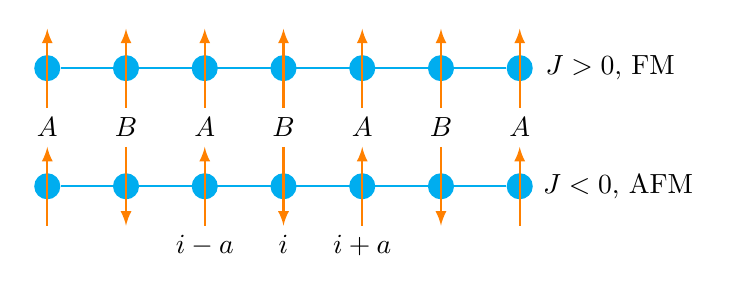
\begin{tikzpicture}
    \node[fill=cyan, circle] (A) at (0, 0) {};
    \node[fill=cyan, circle] (B) at (1, 0) {};
    \node[fill=cyan, circle] (C) at (2, 0) {};
    \node[fill=cyan, circle] (D) at (3, 0) {};
    \node[fill=cyan, circle] (E) at (4, 0) {};
    \node[fill=cyan, circle] (F) at (5, 0) {};
    \node[fill=cyan, circle] (G) at (6, 0) {};
    \draw[thick, cyan] (A) -- (G);
    \draw[-latex, thick, orange] (0, -0.5) -- (0, 0.5);
    \draw[-latex, thick, orange] (1, -0.5) -- (1, 0.5);
    \draw[-latex, thick, orange] (2, -0.5) -- (2, 0.5);
    \draw[-latex, thick, orange] (3, -0.5) -- (3, 0.5);
    \draw[-latex, thick, orange] (4, -0.5) -- (4, 0.5);
    \draw[-latex, thick, orange] (5, -0.5) -- (5, 0.5);
    \draw[-latex, thick, orange] (6, -0.5) -- (6, 0.5);
    \node[] at (7.15, 0) {$J > 0$, FM};

    \node[fill=cyan, circle] (A2) at (0, -1.5) {};
    \node[fill=cyan, circle] (B2) at (1, -1.5) {};
    \node[fill=cyan, circle] (C2) at (2, -1.5) {};
    \node[fill=cyan, circle] (D2) at (3, -1.5) {};
    \node[fill=cyan, circle] (E2) at (4, -1.5) {};
    \node[fill=cyan, circle] (F2) at (5, -1.5) {};
    \node[fill=cyan, circle] (G2) at (6, -1.5) {};
    \draw[thick, cyan] (A2) -- (G2);
    \draw[-latex, thick, orange] (0, -2) -- (0, -1);
    \draw[-latex, thick, orange] (1, -1) -- (1, -2);
    \draw[-latex, thick, orange] (2, -2) -- (2, -1);
    \draw[-latex, thick, orange] (3, -1) -- (3, -2);
    \draw[-latex, thick, orange] (4, -2) -- (4, -1);
    \draw[-latex, thick, orange] (5, -1) -- (5, -2);
    \draw[-latex, thick, orange] (6, -2) -- (6, -1);
    \node[] at (7.25, -1.5) {$J < 0$, AFM};

    \node[] at (0, -0.75) {$A$};
    \node[] at (1, -0.75) {$B$};
    \node[] at (2, -0.75) {$A$};
    \node[] at (3, -0.75) {$B$};
    \node[] at (4, -0.75) {$A$};
    \node[] at (5, -0.75) {$B$};
    \node[] at (6, -0.75) {$A$};

    \node[below] at (2, -2) {$i-a$};
    \node[below] at (3, -2) {$i$};
    \node[below] at (4, -2) {$i+a$};

    % \draw[-latex, very thick] (-1, -1.5) -- (-1, 0);
    % \node[left] at (-1, -0.75) {$B$};
\end{tikzpicture}
\end{document}